\documentclass{beamer}
\usetheme[hideothersubsections]{PaloAlto}
\usecolortheme{albatross}
\usepackage{etoolbox}

\definecolor{Antra}{RGB}{105,105,105}
\definecolor{AntraB}{RGB}{105,105,125}
\definecolor{Gris}{RGB}{80,80,85}
\setbeamercolor*{structure}{fg=Antra!50,bg=AntraB}

\setbeamercolor*{palette primary}{use=structure,fg=white,bg=Gris}
%\setbeamercolor*{palette secondary}{use=structure,fg=white,bg=Gris}


\setbeamercolor*{background canvas}{bg=Antra,fg=Antra}

\setbeamercolor*{normal text}{bg=AntraB,fg=Antra!10}
\setbeamercolor*{navigation symbols}{bg=AntraB,fg=Antra!10}



\beamertemplatenavigationsymbolsempty


\title[Revue de projet Final]{Projet Aéroglisseur \\Revue de Projet Finale}
\author[]{Florian POUTHIER - Tristan DRUSSEL}
\date{Mai 2020}
\institute{4ème année Génie Électrique \\ INSA Strasbourg}
\setbeamertemplate{footline}
{
\leavevmode% 
 \begin{beamercolorbox}[wd=0.3333\paperwidth,left,ht=0.025\paperheight,dp=0.0125\paperheight]{palette primary}
   \hspace*{2em}\insertauthor
 \end{beamercolorbox}
  \begin{beamercolorbox}[wd=0.3333\paperwidth,center,ht=0.025\paperheight,dp=0.0125\paperheight]{AntraB}
 \hspace*{2em}  \insertframenumber\hspace*{2em}
 \end{beamercolorbox}
  \begin{beamercolorbox}[wd=0.3333\paperwidth,right,ht=0.025\paperheight,dp=0.0125\paperheight]{palette primary}
  \insertshorttitle\hspace*{2em}
 \end{beamercolorbox}
  \vskip0pt
}


\begin{document}
\author[]{Tristan DRUSSEL}
	\begin{frame}[noframenumbering,plain]
		\titlepage
	\end{frame}
	\begin{frame}
		\frametitle{Aperçu}
	%Contexte du projet
	%organisation du travail,problématique, questionnement reformulation du rpbleme
		\begin{columns}[T]
	  		\begin{column}{0.5\textwidth}
	  		\begin{itemize}
	  			\item Réalisation d'un aéroglisseur sur la base du Chticat
				\item Mise en oeuvre de l'électronique de puissance, de l'électronique numérique et de la mécanique
	  		\end{itemize}
	    	
	  		\end{column}
	  		\begin{column}{0.5\textwidth}
	  			\begin{figure}
	    			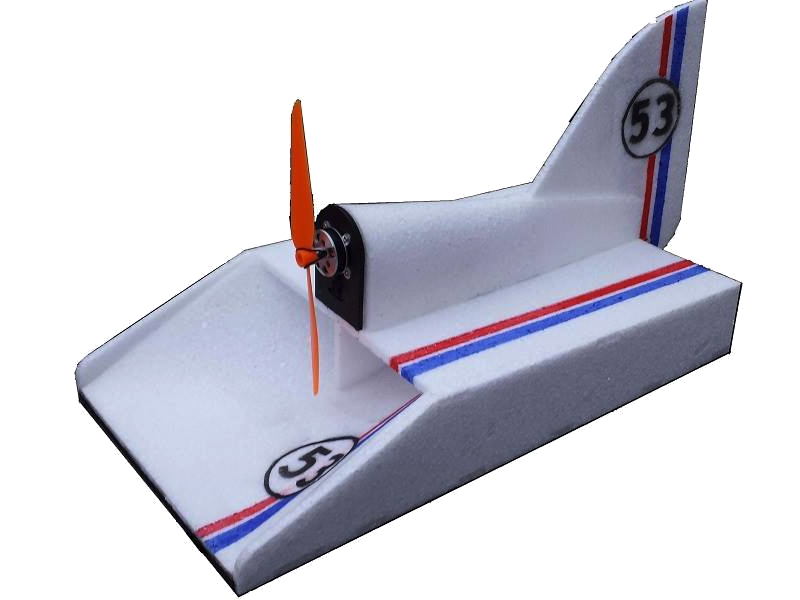
\includegraphics[width=0.8\textwidth]{"../Illus/Chticat.png"}
	    			\caption{Photo d'un Chticat originel}
	    		 \end{figure}
	  		\end{column}
		\end{columns}
	\end{frame}
	\begin{frame}{Sommaire}
	%Plan d'intervention succinct
		\setcounter{tocdepth}{1}
		\tableofcontents
	\end{frame}
	\begin{frame}{L'aspect mécanique}
		\section[Mécanique]{L'aspect Mécanique}
		\subsection{Modèle CAO}
		\begin{columns}[T]
	  		\begin{column}{0.5\textwidth}
		    	\begin{itemize}
		    		\item Récupération des sources
		    		\item Adaptation du modèle
		    	\end{itemize}
	  		\end{column}
	  		\begin{column}{0.5\textwidth}
	    		\begin{figure}
	    			\includegraphics[width=0.8\textwidth]{"../Illus/3Dview.png"}
	    			\caption{Modèle 3D modifié et adapté}
	    		 \end{figure}
	  		\end{column}
		\end{columns}
		
	\end{frame}
	\begin{frame}{Électronique Numérique}
		\section[ENUM]{L'aspect Électronique Numérique}
		Communication entre différents éléments:
		\begin{itemize}
			\item Application mobile
	  		\item Module Bluetooth: \texttt{HC-05}
			\item \texttt{PIC16F1619}
			\item \texttt{dsPIC10F2030}
	  	\end{itemize}
	  	Contrôle de l'onduleur
	\end{frame}
	\begin{frame}{Électronique Numérique:\\Communication Bluetooth}
		\subsection[Bluetooth]{Communication Bluetooth}
		\begin{columns}[T]
	  		\begin{column}{0.5\textwidth}
		    	\begin{itemize}
		    		\item Contrôle à partir du Smartphone
		    	\end{itemize}
		    	\begin{figure}
		    		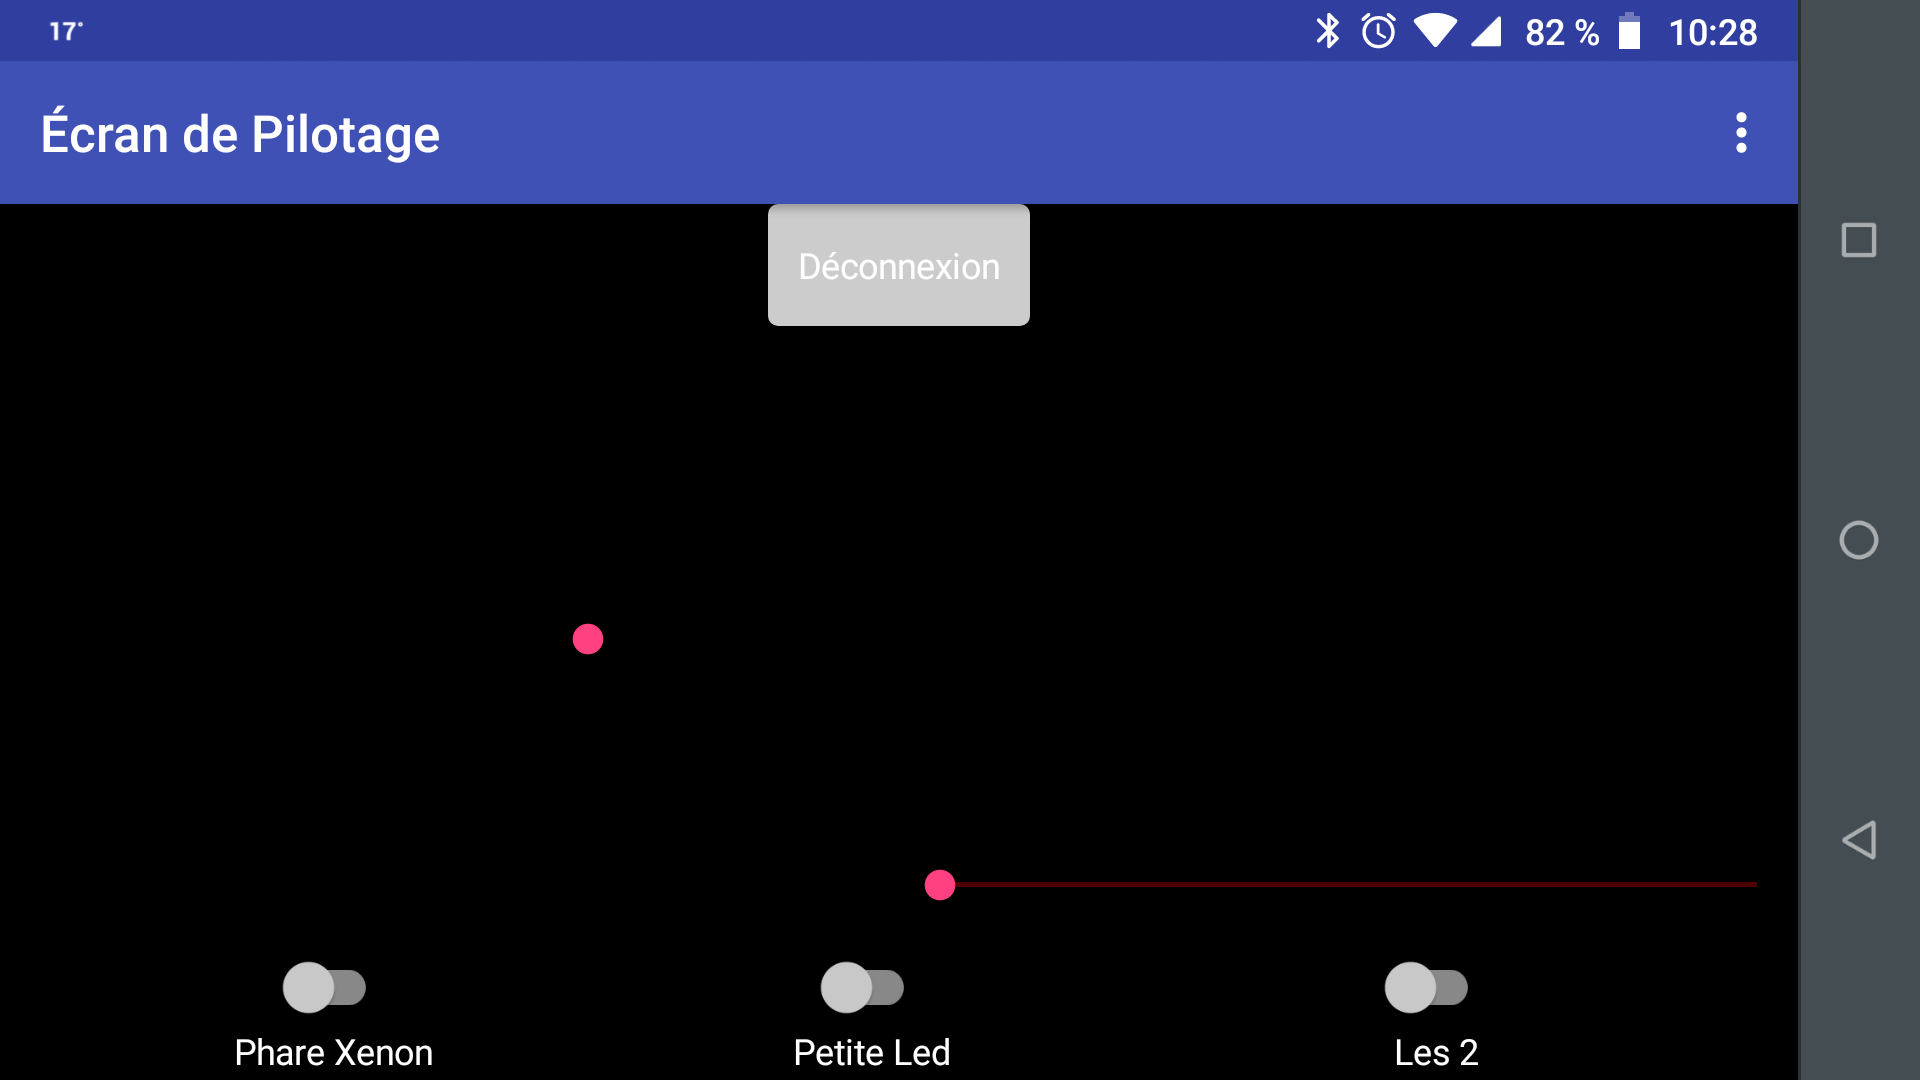
\includegraphics[width=0.8\textwidth]{"../Illus/AppPilotage.png"}
	    			\caption{Ecran de pilotage de l'application}
	    		 \end{figure}
	  		\end{column}
	  		\begin{column}{0.5\textwidth}
	  			\begin{figure}
	    			\hspace*{2em}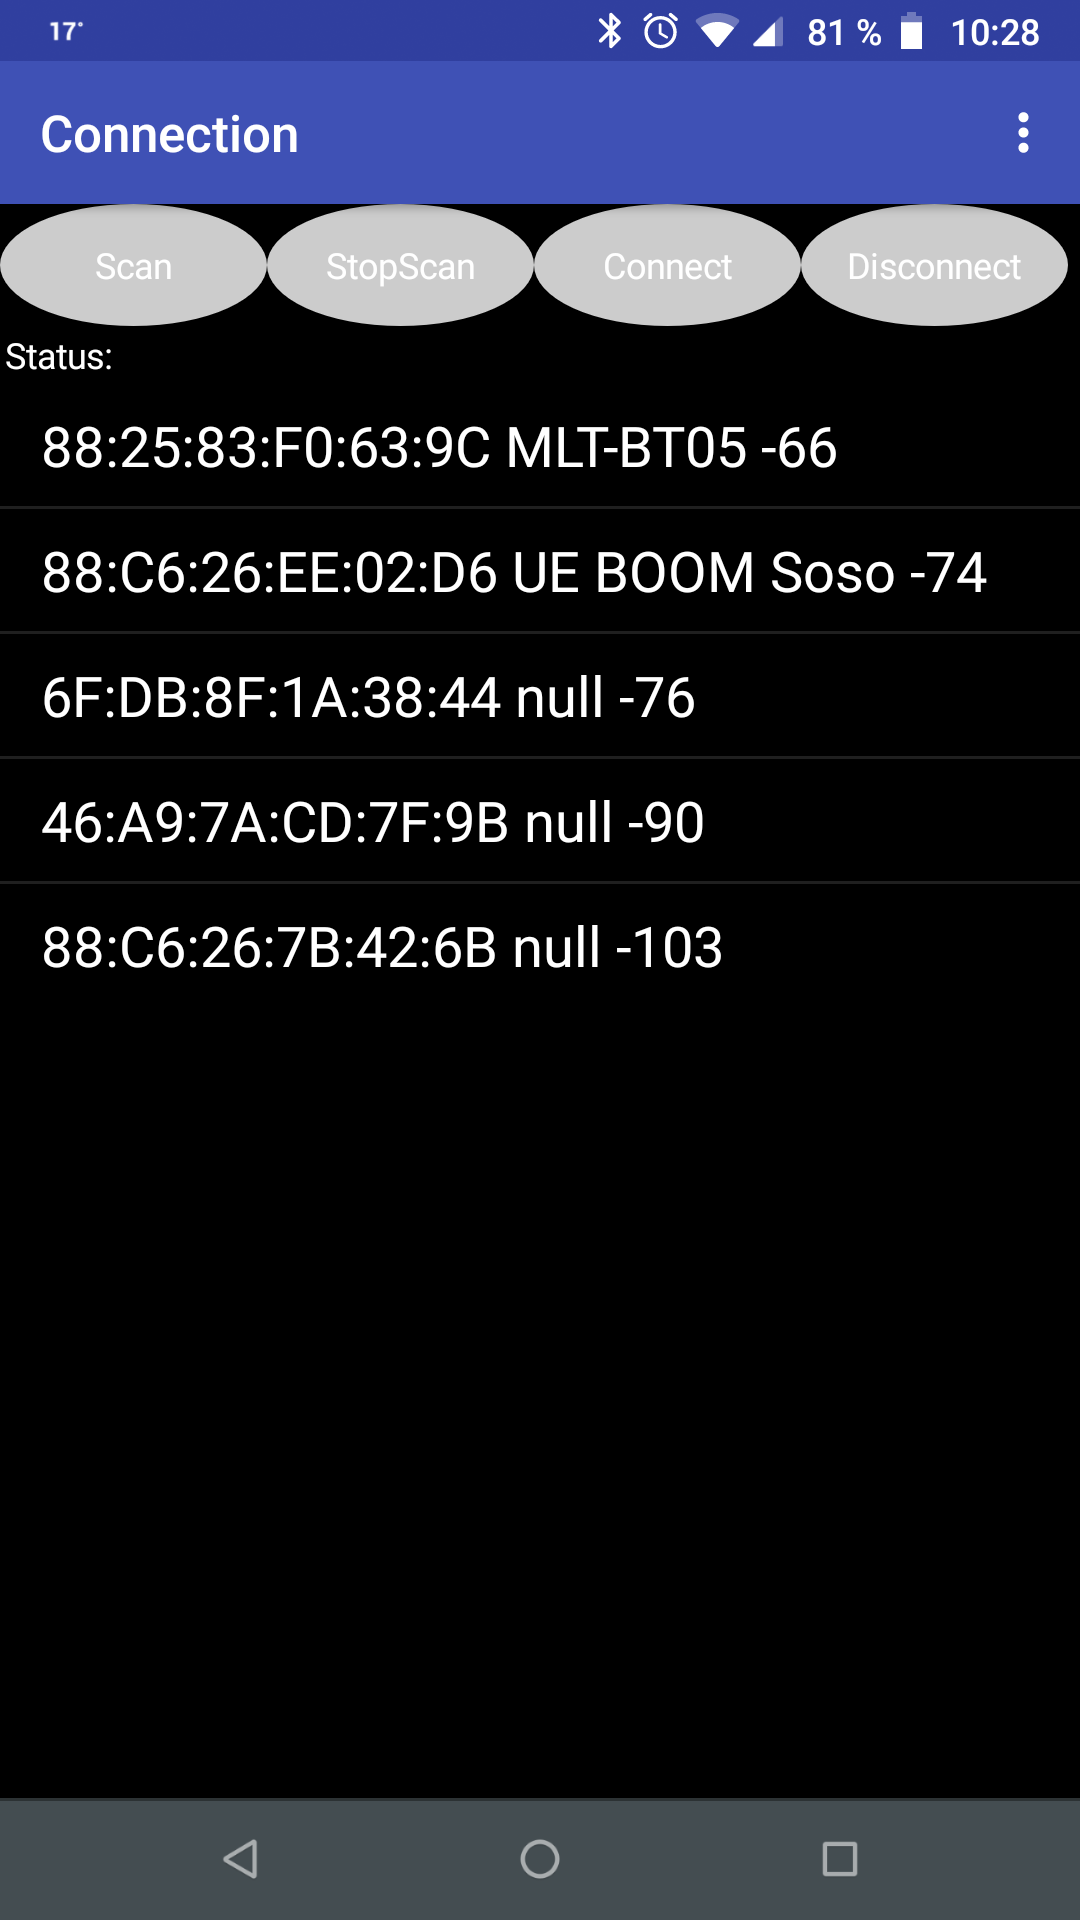
\includegraphics[height=0.8\textheight]{"../Illus/AppConnection.png"}
	    			\caption{Ecran de connection de l'application}
	    		\end{figure}
	  		\end{column}
		\end{columns}
		
	\end{frame}
	\begin{frame}{Électronique Numérique:\\Communication Série}
		\subsection[Série]{Communication Série}
		\begin{itemize}
		    \item Communication entre le Récepteur Bluetooth et le \texttt{PIC16F1619}
		\end{itemize}
	\end{frame}
	\begin{frame}{Électronique Numérique:\\Communication \textit{Serial Peripheral Interface}}
		\subsection[SPI]{Communication SPI}
		\begin{itemize}
		    \item Communication entre le \texttt{PIC16F1619} et le \texttt{dsPIC10F2030}
		\end{itemize}
	\end{frame}
	\author[]{Florian POUTHIER}
	\begin{frame}{Électronique de Puissance}
		\section[ENPU]{L'aspect Électronique de Puissance}
		
		
	\end{frame}
	\begin{frame}
		\section[Poursuites]{Poursuites du projet}
	\end{frame}
	
	\begin{frame}{Conclusion}
	\section*{Conclusion}
	%Conclusion
	\end{frame}
	\begin{frame}{Bibliographie}
	\section*{Bibliographie}
		\bibliographystyle{plain} 
		\bibliography{../Etude/biblio.bib}
	\end{frame}
	\begin{frame}[plain]{Merci de votre attention}
	\section*{}
		%remerciement
		\titlepage
	\end{frame}
\end{document}